\part{Álgebra Lineal}

\begin{myexampleblock}{Álgebra Lineal}



\vspace{2mm}  Se denomina álgebra a la rama de las matemáticas que se orienta a la generalización de las operaciones aritméticas a través de signos, letras y números. En el álgebra, las letras y los signos representan a otra entidad a través de un simbolismo.

\vspace{2mm} Lineal, por su parte, es un adjetivo que refiere a lo vinculado a una. En el ámbito de la matemática, la idea de lineal alude a aquello que cuenta con consecuencias que son proporcionales a una causa.

\vspace{2mm} Se conoce como álgebra lineal a la especialización del álgebra que trabaja con matrices, vectores, espacios vectoriales y ecuaciones de tipo lineal. Se trata de un área del conocimiento que se desarrolló especialmente en la década de 1840 con los aportes del alemán Hermann Grassmann (1809-1877) y el irlandés William Rowan Hamilton (1805–1865), entre otros matemáticos.

\vspace{2mm} Los espacios vectoriales son estructuras que surgen cuando se registra un conjunto que no está vacío, una operación externa y una operación interna. Los vectores son los elementos que forman parte del espacio vectorial. En cuanto a las matrices, se trata de un conjunto bidimensional de números que permiten la representación de los coeficientes que tienen los sistemas de ecuaciones lineales.

\vspace{2mm} William Rowan Hamilton es uno de los nombres más destacados del ámbito de las matemáticas, ya que fue quien acuñó el término «vector», además de haber creado los cuaterniones. Este concepto se extiende de los números reales, así como ocurre con los complejos. Los cuaterniones no son únicamente una curiosidad algebraica, tienen diversas aplicaciones físicas dentro del electromagnetismo, teoría de la relatividad y mecánica cuántica, entre otras.


\vspace{2mm} Siguiendo con la definición de los elementos con los que trata el álgebra lineal, es importante saber que un sistema de ecuaciones lineales se compone de ecuaciones de primer grado, definidas sobre un anillo conmutativo o un cuerpo. Todos estos conceptos (espacio vectorial, cuerpo, anillo, grupo) son las llamadas `estructuras algebraicas’ y formarán nuestro primer tema.

\vspace{2mm} Los espacios vectoriales, el foco de estudio del álgebra lineal, cuentan con dos conjuntos: uno de vectores y otro de escalares. Los escalares son elementos de los cuerpos matemáticos que se usan para llevar a cabo la descripción de un fenómeno con magnitud, aunque sin dirección; puede ser un número real o complejo.

\vspace{2mm} El álgebra lineal es un instrumento de gran aplicación en casi todas las ramas de la matemática moderna, también muy utilizado en disciplinas como la física, computación e ingeniería entre otras; orienta su estudio y enseñanza sobre las bases teóricas y prácticas de: vectores, álgebra de matrices, cálculo de raíces, determinantes, sistemas de ecuaciones lineales, espacios vectoriales y sus respectivas transformaciones. 

\vspace{2mm} 
.
	
\end{myexampleblock}




\chapter{Estructuras algebraicas básicas $\divideontimes$} \label{e_alg}	
\chaptermark{Estructuras algebraicas}
\section{Operación Interna}
\begin{defi}
Dados tres conjuntos $A$, $B$ y $C$, se llama `ley de composición' en los conjuntos $A$ y $B$ y resultado en el conjunto $C$, que denotaremos por $\oplus$, a una aplicación: 
\begin{equation*}
	\oplus: A \times B \longrightarrow C: \qquad \therefore \qquad (a,b) \leadsto a \oplus b = c \in C
\end{equation*}	
\end{defi}
\begin{defi}
Dada $\oplus: A \times B \to C$, decimos que esta ley de composición es `interna' si $A=B=C$. También se le llama `operación binaria interna' o, más abreviadamente, `operación interna'.
\end{defi}
\begin{ejem}
La suma y productos ordinarios en $\mathbb R$, usualmente denotados por $+$ y $\cdot$, son leyes de composición interna.
\begin{equation*}
	\begin{split} 
		+:\; \mathbb R \times \mathbb R \longrightarrow \mathbb R & (x,y) \leadsto x+y \in \mathbb R \\
		\cdot : \;  \mathbb R \times \mathbb R \longrightarrow \mathbb R & (x,y) \leadsto x \cdot y \in \mathbb R
	\end{split}
\end{equation*}	
\end{ejem}
\begin{ejem}
La resta no es una operación interna en $ \mathbb N$, ya que, por ejemplo, $4,7 \in  \mathbb N,$, pero $4-7=-3 \notin  \mathbb N$.

Análogamente, la división no es una operación interna en ninguno de los conjuntos numéricos habituales ($\, \mathbb N \subset \mathbb Z \subset \mathbb Q \subset \mathbb R \subset \mathbb C\,$) ya que no está definida la división por $0$ en ninguno de ellos.
\end{ejem}
\begin{defi}
Dados dos conjuntos $A$ y $B$, se llama `ley de composición externa' a una aplicación de $A\times A$ en $B$ tal que a todo par de elementos de $A$ les asocia un elemento de $B$.	
\end{defi}
\begin{ejem}
La resta de números naturales del ejemplo anterior es una operación externa de $\mathbb N \times \mathbb N \to \mathbb Z$.	
\end{ejem}
\begin{defi}
Una aplicación $\odot: \; A \times B \to A \therefore (a,b) \leadsto c=a\odot b \in A$, se llama `ley de composición externa por la derecha'. A los elementos del conjunto $B$ se les llama multiplicadores o `escalares'.

Si se tiene:  $\odot: \; B \times a \to A \therefore (b,a) \leadsto c=b\odot a \in A$, se dice que es una `ley de composición externa por la izquierda'.
\end{defi}
\begin{ejem}
Un ejemplo de operación externa es `el producto de un vector por un escalar' (o número real). Si $V$ es el conjunto de vectores libres del plano, el producto $\lambda \cdot \vec{v} \in V; \; \lambda \in \mathbb R \text{ y } \vec{v} \in V$  es una operación externa. \textcolor{gris}{Por ejemplo, $\vec{v}=(2,3) \to 4\cdot (2,-3)=(8,-12)$}.

Otro ejemplo de operación externa es el producto de un número real por una función (real de variable real). Si $\mathcal F$ es el el conjunto de funciones reales de variable real, la operación $\; \cdot:\; \mathbb R \times \mathcal F \to \mathcal F$, tal que $(k\cdot f)(x)=k\cdot f(x) \in \mathcal F$, con $k \in \mathbb R$ y $f \in \mathcal F$, también es una operación externa.
\end{ejem}
\noindent \textbf{Propiedades.} Las leyes de composición no tienen por qué satisfacer ningún requisito en general, pero serán interesantes aquellas que verifiquen ciertas propiedades.

Las propiedades más interesantes que pueden cumplir las leyes de composición interna, son:

\begin{itemize}
\item \textbf{Asociativa:} $a \oplus (b \oplus c) =(a \oplus b) \oplus c; \; \; \forall a,b,c \in A$

La propiedad asociativa, si se cumple, es la que nos permit prescindir de los paréntesis.

\item \textbf{Conmutativa:} $a \oplus b = b \oplus a; \; \; \forall a,b \in A$	

\item \textbf{Distributivas:} Dado el conjunto A y las operaciones internas $\oplus, \odot$:
	\begin{itemize}
	 
	\item Se dice que $\odot$ es `distributiva por la izquierda' respecto de $\oplus$ si: 

	$a \odot (b \oplus c) =(a \odot b)\oplus(a \odot c); \; \; \forall a,b,c \in A$

	\item Se dice que $\odot$ es `distributiva por la derecha' respecto de $\oplus$ si: 

	$(a \oplus b) \odot c =(a \odot c)\oplus(b \odot c); \; \; \forall a,b,c \in A$

	\item Se dice que $\odot$ es `distributiva' respecto de $\oplus$ si lo es por la izquierda y por la derecha, es decir:

	$(a\oplus b)\odot(c\oplus d)=(a \odot c) \oplus (a \odot b) \oplus(b \odot c) \oplus(b \odot d); \; \; \forall a,b,c,d \in A $
	\end{itemize}

\item \textbf{Elemento Neutro:} Decimos que la operación interna $\oplus$ tiene `elemento neutro' en $A$, si:
$\exists e \in A \; / \;  e\oplus a + a \oplus e = a; \; \; \forall a \in A$ 

\textcolor{gris}{Al elemento neutro lo denotamos por $e$.}

\item \textbf{Elemento Simétrico:} Dada una operación interna $\oplus$ en un conjunto $A$ con elemento neutro $e$, se llama `elemento simétrico', \textit{si existe}, del elemento $a$ a un elemento $\overline{a} \in A$ tal que:
$\; \; a \oplus \overline{a} = \overline{a} \oplus a =e$

\textcolor{gris}{Para la suma ordinaria en $\, \mathbb N \subset \mathbb Z \subset \mathbb Q \subset \mathbb R \subset \mathbb C\,$, el elemento neutro es el ``$0$'' y el ``$1$'' lo es para el producto ordinario.}

\textcolor{gris}{Para la suma ordinaria, el simétrico de un elemento $x$ es $-x$ y se le llama `elemento opuesto'. En el producto ordinario, para un elemento $n \neq 0$, el simétrico es $\frac 1 x$ y se le llama 'elemento inverso'.}

\textcolor{gris}{Para la composición de funciones reales de variable real, el elemento neutro es la función identidad $I(x)=x$ y el simétrico de una función (inyectiva) es la función inversa ($\;(f \circ f^{-1}=I=f^{-1} \circ f \;$.}

\item \textbf{Elemento regular o simplificable:} Decimos que $a\in A$ es `regular' o `simplificable' para la composición interna $\oplus$ si se verifica:

\hspace{10mm} Si $\; a\oplus a_1 = a \oplus a_2 \Rightarrow a_1=a_2; \;\;  \forall a_1, a_2 \in A\; $, y

\hspace{10mm} Si $\; a_1\oplus a = a_2 \oplus a \Rightarrow a_1=a_2; \;\;  \forall a_1, a_2 \in A\; $

\end{itemize}


\begin{defi}
Se llama `estructura algebraica' a un conjunto A y unas operaciones  $\oplus, \odot, \otimes, \cdots$, internas o externas, definidas en $A$, de modo que se verifican ciertas propiedades. Se denota por: $A(\oplus, \odot, \otimes, \cdots)$.

A continuación se describen las estructuras algebraicas más habituales y que son necesarias para llegar, en un próximo tema, a la estructura de `espacio vectorial'.
\end{defi}

\section{Grupos}

\begin{defi}
Llamamos `grupo' a una estructura algebraica $(G,\otimes)$	que verifica las propiedades:

\begin{enumerate}
\item Asociativa: $\; x\otimes (y \otimes z)=(x \otimes y) \otimes z; 	\; \; \forall x,y,z \in A$
\item Existencia de Neutro: $\;  \; \exists \; e\in A \; / \; x \otimes e = e \otimes x = x, \; \forall x\in A$	
\item Existencia de simétrico: $\; \forall x \in A,\; \exists \; y\in G\; / \; x \otimes y = y \otimes x = e$
\end{enumerate}
\end{defi}

\begin{defi}
Si el grupo $(G,\otimes)$ cumple también la propiedad conmutativa:
$\; \; x \otimes y = y \otimes x; \; \; \forall x,y \in G \; \; $,
se dice de el `grupo es conmutativo o Abeliano'. 
\end{defi}
\begin{ejem}
	En el grupo $(\mathbb R, +)$, el neutro es $0$ y el simétrico (opuesto) de $x$ es $-x$. En $\mathbb R^*=\mathbb R \sim \{0\}, \cdot)$, el neutro es el $1$ y el simétrico (inverso) de $x$ es $\frac 1 x$. Ambos grupos son conmutativos. Además:
	\vspace{-2mm}
	\begin{enumerate}
	\item $\mathbb N, \mathbb Z, \mathbb Q, \mathbb R, \mathbb C$son grupos abelianos respecto de la suma ordinaria.
	\item Los conjuntos 	$\mathbb Q \sim \{0\}, \mathbb R \sim \{0\}, \mathbb C \sim \{0\}$ son grupos abelianos respecto del producto ordinario.
	\item El conjunto de las funciones reales de variable real, $\mathcal F$, respecto de la suma de funciones, también tiene estructura de grupo abeliano. Así como el conjunto de los vectores libres del plano $V$ y la suma de éstos.
	\end{enumerate}
\end{ejem}

\section{Anillos}
\begin{defi} Un `anillo' es una estructura algebraica formada por un conjunto y dos leyes de composición interna, $\; (A,\oplus, \odot)\; $, que verifican las siguientes propiedades:
\begin{enumerate}
	\item $\; (A,\oplus)\;$ es un grupo abeliano. Su elemento neutro lo denotaremos por $0$.
	\item $\odot$ cumple la asociativa: $\; (x\odot y)\odot z=x \odot(y \odot z), \; \; \forall x,y,z \in A$	
	\item $\; \left. \begin{matrix}
	x\odot (y \oplus z)=(x\odot y)\oplus(x \odot z)\\
	(x\oplus y)\oplus z= (x \odot z)\oplus (y \odot z)
\end{matrix} \right\} \; \; \begin{matrix}
\text{distributivas de } \odot \\ 
\text { respecto de } \oplus 	\\
\forall x,y,z \in A
 \end{matrix}$
\end{enumerate}
\end{defi}	
\begin{defi}
$(A,\oplus, \odot)\; $ es anillo `unitario' si se verifica que:

$\exists \; \overline{e} \; \in A \; / \; x\odot \overline{e} = \overline{e} \odot x = x, \; \forall x \in A$	(existe neutro para la segunda ley de composición).
\end{defi}
\begin{defi}
$(A,\oplus, \odot)\; $ es anillo `conmutativo' si se verifica que:

$x\odot y = y \odot x, \; forall x,y \in A\; $	(la segunda ley es conmutativa).
\end{defi}
\begin{defi}
Un elemento $x$ de un anillo unitario 	$\; (A,\oplus, \odot)\; $ se dice `inversible' si posee simétrico respecto de la segunda ley, $\odot$, es decir:

$ \exists \; y \in A\; / \; x\odot y=y\odot x = \overline{e}$
\end{defi}
\begin{ejem}
En $\;(\mathbb Z, +, \cdot )\;$	, los únicos elementos invertibles son el $1$ y el $-1$.

En $\;(\mathbb R, +, \cdot )\;$	, el único elementos no invertibles es el $0$.

$(\mathbb Z, +, \cdot )\;$	es un anillo conmutativo unitario, $\;(\mathbb Q, +, \cdot )\;$, 	$\;(\mathbb R, +, \cdot )\;$	, $\;(\mathbb C, +, \cdot )\;$	son anillos conmutativos unitarios en los que el único elemento no invertible es el $0$

En determinados anillos es posible encontrar dos elemento no nulos que, al operarlos mediante la segunda ley (que habitualmente denominamos producto), se obtiene el elemento neutro de la primera ley (el $0$ habitualmente). Es decir, se pueden multiplicar dos elementos distintos de $0$ y que el resultado sea $0$. A estos elemento se les conoce como `divisores de cero'. 

Por ejemplo: el anillo $(\mathbb Z^2=\mathbb Z \times \mathbb Z,\;  \; +,\;   \cdot \; )$ con las leyes de composición $(x_1,y_1)+(x_2,y_2)=(x_1+x_2, y_1+y_2)$ y $(x_1,y_1)\cdot (x_2,y_2)=(x_1\cdot y_1, x_2\cdot y_2)$, los elementos $(1,0)$ y $(0,1)$ son `divisores de cero', ya que: $(1,0)\cdot (0,1)=(0,0)$.

A los anillos que no tienen divisores de cero, es decir: $\forall x,y \in A: \; x \cdot y =0 \Leftrightarrow x=0 \; vee \; y=0$, se les llama `anillos íntegros o dominio de integridad'. $(\mathbb Z, +, \cdot )\;(\mathbb Q, +, \cdot )\;$, 	$\;(\mathbb R, +, \cdot )\;$	, $\;(\mathbb C, +, \cdot )\;$, con las leyes habituales de suma y producto, son `dominios de integridad'.
\end{ejem}



\section{Cuerpos}
\begin{defi}
Se llama `cuerpo' a todo anillo unitario $(K,\oplus,\odot)$, tal que $(K\sim\{0\},\odot)$ es un grupo, es decir, todo elemento $x\in K, \; x\neq 0$ es inversible respecto de $\odot$.

Si el anillo $(K\sim\{0\},\odot)$ es conmutativo, se dice que el cuerpo $K$ es conmutativo.
\end{defi}
\begin{ejem}
Los conjuntos $\mathbb Q, \mathbb R, \mathbb C$, respecto de las operaciones ordinarias, son cuerpos conmutativos.	
\end{ejem}

\section{Espacios vectoriales}
El concepto de `espacio vectorial' se verá con más detalle en un próximo tema. Dejamos ahora solo su definición:
\begin{defi}
	Un conjunto $V$ tiene estructura de `espacio vectorial' sobre un cuerpo $K$ si:
	
	--- En $V$ hay definida una ley de composición interna (suma) que da a $V$ estructura de `grupo abeliano'.
	
	--- En $V$ hay definida una ley de composición externa (producto por un escalar, elemento del cuerpo $K$) tal que: $\forall u \in V ,\; \forall \lambda \in K \leadsto k\cdot u=ku \in V$, que verifica las siguientes leyes:
	
	\begin{multicols}{2}
	\begin{enumerate}
	\item $\lambda (u+v)=\lambda u + \lambda v$
	\item $(\lambda + \mu)u=\lambda u + \mu u$
	\item $\lambda(\mu u)=(\lambda \mu) u$
	\item $1u=u \quad$ \footnotesize{$( \forall u,v \in V, \forall \lambda, \mu \in K)$}	
	\end{enumerate}
	\end{multicols}	
\end{defi}

%\vspace{25mm}

	\begin{figure}[H]
		\centering
		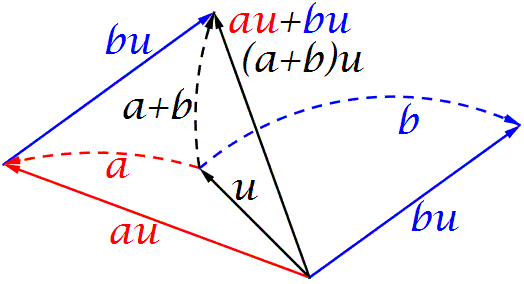
\includegraphics[width=.8\textwidth]{imagenes/imagenes01/T01IM01.png}
	\end{figure}


\section{Ejercicios resueltos}

\begin{ejre} Considera la ley de composición: $a \oplus b=\sqrt[3]{a^3+b^3}$, con $, b\; \in \; \mathbb R$. Demuestra que $(R,\oplus)$ es grupo abeliano.
\end{ejre}

\begin{proofw}\renewcommand{\qedsymbol}{$\diamond$}

\noindent 1) $\oplus$ interna: $a,b\in \mathbb R \to 	a\oplus b=\sqrt[3]{a^3+b^3} \in \mathbb R$ 

\noindent 2) $\oplus$ asociativa: $(a \oplus b) \oplus c = \sqrt[3]{a^3+b^3} \oplus c = \sqrt[3]{(\sqrt[3]{a^3+b^3})^3+c^3}=\sqrt[3]{a^3+b^3+c^3}\; ; \qquad a\oplus(b \oplus c)= a \oplus \sqrt[3]{b^3+c^3} = \sqrt[3]{a^3+(\sqrt[3]{b^3+c^3})^3}= \sqrt[3]{a^3+b^3+c^3}$

\noindent 3) $\oplus$ neutro: $a+e=\sqrt[3]{a^3+e^3}=a=\sqrt[3]{a^3}\to e=0$

\noindent 4) $\oplus$ simétricos: $a\oplus \overline{a}=e \to \sqrt[3]{a^3+{\overline a}^3}=0 \to {\overline{a}}^3=-a^3 \to \overline{a}=-a$

\noindent 5) $\oplus$ conmutativa: $a \oplus b=\sqrt[3]{a^3+b^3}=\sqrt[3]{b^3+a^3}=b \oplus a$

Efectivamente, $\boldsymbol{(R,\oplus)}$ es \textbf{grupo comutativo.}
\end{proofw}

\begin{ejre} Considera las leyes de composición: $a\oplus b=a+b-8; \quad a \otimes b= a+b-ab$, demuestra que $(\mathbb Z, \oplus, \otimes)$ es un anillo.	
\end{ejre}

\begin{proofw}\renewcommand{\qedsymbol}{$\diamond$}

\noindent 1) $\oplus$ interna: 	$a,b\in \mathbb Z \to a+b-8 \in \mathbb Z$

\noindent 2) $\oplus$ asociativa: $(a\oplus b)\oplus c = (a+b-8)\oplus c= (a+b-8)+c-8= a+b+c-16; \qquad a\oplus(b\oplus c)=a\oplus(b+c-8) a+(b+c-8)-8=a+b+c-16$ 

\noindent 3) $\oplus$ neutro: $a\oplus e=a+e-8=a \to e=8$

\noindent 4) $\oplus$ simétrico: $a\oplus \overline{a}=a+\overline{a}-8=e=8 \to \overline{a}=16-a$

\noindent 5) $\oplus$ conmutativa: $a\oplus b=a+b-8 = b+a-8=b\oplus a$

\noindent 6) $\otimes$ interna: $a,b \in \mathbb Z a\otimes b =\to a+b-ab \in \mathbb Z$

\noindent 7) $\otimes$ asociativa:

$(a\otimes b)\otimes c= (a+b-ab)\otimes c =(a+b-ab)+c-(a+b-ab)c=a+b+c-ab-ac-bc+abc$

\centerline{$=$}

$a\otimes(b\otimes c)=a\otimes (b+c-bc)= a+(b+c-bc)-a(b+c-bc)=a+b+c-ab-ac-bc+abc$

\noindent 8) distributiva de $\otimes$ respecto de $\oplus$:

$a\otimes (b\oplus c)=  a\otimes (b+c-8)= a+(b+c-8)-a(b+c-8)=a+b+c-8-ab-ac+8a=9a+b+c-ab-ac-8$

\centerline{$\neq$}

$(a\times b) \oplus (a \otimes c)= (a+b-ab) \oplus (a+c-ac) = (a+b-ab)+(a+c-ac)-8=2a+b+c-ab-ac-8$

No se cumple la propiedad distributiva, luego  $\boldsymbol{(\mathbb Z, \oplus, \otimes)}$ \textbf{no es un anillo}.	

\end{proofw}


\begin{ejre}
	Demuestra que $(\mathbb C,+,\cdot)$, con las leyes usuales de suma y producto de números complejos es un `cuerpo conmutativo'.
\end{ejre}

\begin{proofw}\renewcommand{\qedsymbol}{$\diamond$}
	Recuérdese que un cuerpo es un anillo con elemento inverso para la  segunda ley para todos los elementos de $\mathbb C$ excepto en neutro de la primera ley. Además el cuerpo es conmutativo si lo es la segunda ley. Si antes comprobábamos 8 propiedades, ahora serán 10.
	
	$z\in \mathbb C \; / \; z=a+bi \text{ con } a,b\in \mathbb R; \; i=\sqrt{-1} \notin \mathbb R \; (i^2=-1)$. $a$ es la `parte real' y $b$ la `parte imaginaria', ambas reales.
	
	En lo que sigue, $z_k=a_k+b_k\; i, \; k=\{1,2,3\}; a_k, b_k \in \mathbb R$
	
\noindent 1) $+$ es interna:	 $z_1+z_2=(a_1+b_1 i)+(a_2+b_2 i)=(a_1+a_2)+(b_1+b_2)\;i \; \in \mathbb C$

\noindent 2) $+$ asociativa: $z_1+(z_2+z_3)=(a_1+b_1)\; i + [(a_a+b_2\; i)+ (a_3+b_3)\; i]=\cdots= (a_1+a_2+a_3) + (b_1+b_2+b_3)\; i =\cdots= [(a_1+b_1\; i)+ (a_2+b_2\;i)]+ (a_3+b_3\; i)= (z_1+z_2)+z_3$

\noindent 3) $+$ neutro: $z+e=z \to (a+bi)+ 0 = a+bi \Rightarrow e=0=0+0i$

\noindent 4) $+$ simétrico (opuesto): $z+(-z)=0 \to (a+bi)+ (-z)=0 \Rightarrow -z=-a-bi$

\noindent 5) $+$ conmutativa: $z_1+z_2= (a_1+b_1i)+(a_2+b_2i)=(a_1+a_2)+(b_1+b_2)i=(a_2+a_1)+(b_2+b_1)i=z_2+z_1$

\noindent 6) $\cdot$ interna: $z_1\cdot z_2=(a_1+b_1i)\cdot(a_2+b_2 i)=a_1a_2+a_1b_2i+b_1a_2i+b_1b_2\cancelto{-1}{i^2}=(a_1a_2-b_1b_2)+(a_1b_2+a_2b_1)\;i \in \mathbb C$

\noindent 7) $\cdot$ asociativa:

$z_1\cdot(z_2\cdot z_3)=(a_1+b_1i)\cdot [(a_2a_3-b_2b_3)+(a_2b_3+a_3b_2)\; i]= [a_1(a_2a_3-b_2b_3)-b_1(a_2b_3+a_3b_2)] + [a_1(a_2b_3+a_3b_2)+b_1(a_2a_3-b_2b_3)]\; i \cdots \to$

\centerline{compruébese que son $=$}

$(z_1\cdot z_2)\cdot z_3= [(a_1a_2-b_1b_2)+(a_1b_2+a_2b_1)\;i]\cdot (a_3+b_3i)= \cdots \to $

\noindent 8) $\cdot$ distributiva respecto de $+$:

$z_1\cdot(z_2+z_3)=(a_1+b_1i)\cdot [(a_2+a_3)+(b_2+b_3)\; i] = \cdots \to $

\centerline{compruébese que son $=$}

$(z_1\cdot z_2)+(z_1\cdot z_3)=[(a_1a_2-b_1b_2)+(a_1b_2+a_2b_1)\; i] +  [(a_1a_3-b_1b_3)+(a_1b_3+a_3b_1)\; i] = \cdots \to $ 

\noindent 9) $\cdot$ simétrico (inverso): El neutro en el producto es $1=1+0i; \; z\cdot 1 =(a+bi)(1+0i)=a+bi$

$\forall z\neq 0 \in \mathbb C, \; z=a+bi, \; \exists z^{-1}=\frac 1 z\; / \; z\cdot z^{-1}=1$

En efecto si $z\cdot z^{-1}=1 \to z^{-1}= \frac 1 z = \frac {1}{a+bi}$
\textcolor{gris}{$\cdot \frac {a-bi}{a-bi}$}
$= \frac {a-bi}{a^2-b^2}= \frac {a}{a^2-b^2} + \frac {-b}{a^2+b*2} \; i \in \mathbb C$

\noindent 10) $\cdot$ conmutativa: $z_1\cdot z_2=(a_1+b_1i)\cdot(a_2+b_2 i)=(a_1a_2-b_1b_2)+(a_1b_2+a_2b_1)\;i = (a_2a_1-b_2b_1)+(a_2b_1+a_1b_2)\;i= (a_2+b_2i)\cdot (a_1+b_1i)=z_2\cdot z_1$

\end{proofw}



\begin{myexampleblock}{Comentarios sobre los números complejos.}

\small{El nombre escogido, `números complejos',  para estos números tiene lo suyo, pero ... sigamos adelante.}

\vspace{2mm}
\small{Estos extraños números surgen de la mano de Cardano y Tartaglia en el s. XVI, cuando intentaban resolver ecuaciones de tercer grado. Se dieron cuenta que necesitaba considerar las raíces cuadradas de números negativos, así, p.e., para calcular $\sqrt{-25}$ hacían lo siguiente: $\sqrt{-25} = \sqrt{ 25 \cdot (-1)} = \pm 5 \; \sqrt{-1}$}


\vspace{2mm}
\small{En el s. XVII, Leibniz considera a la $\sqrt{-1}$ como una especie de `anfibio entre el ser y la nada'. Los matemáticos y físicos de la época usan estos números pero con desconfianza.}


\vspace{2mm}
\small{Euler, en el s. XVIII bautiza a $\sqrt{-1}$ como $i$ (de número imaginario). Ahora, las raíces de números negativos son algo tan sencillo como $\sqrt{-4}=\pm 2\;i$}


\vspace{2mm}
\small{A finales del s. XVIII, Euler demuestra su famoso TEOREMA FUNDAMENTAL DEL ÁLGEBRA, que asegura que todo polinomio de grado $n$ tiene, exactamente, $n$-raíces (considerando la multiplicidad y estas imaginarias).  Así, p.e., la ecuación                 $x^2-4x+13=0$ tiene por soluciones  $2+3i$  y  $2-3i$.}


\vspace{2mm}
\small{A partir del s. XIX, Gauss logra la representación gráfica de estos números complejos y su interpretación geométrica. Desde entonces son aceptados sin reservas.}


\vspace{2mm}
\small{s. XXI. La aplicación de los números complejos está presente en muchos apartados de las ciencias.}

\vspace{2mm}
\small{--- En electrónica la ley de ohm ($IR=V$) para corriente alterna necesita de los números complejos: $IZ=V; \; Z=R+iX$  ($Z$ impedancia, tiene parte real o resistiva $R$ y parte imaginaria o reactancia $X$)}

\vspace{2mm}
\small{También se usan los números complejo en electromagnetismo (las ondas e.m. son complejas) y en física cuántica (la amplitud de probabilidad es compleja, su cuadrado es lo observable).}


\vspace{2mm}
\small{--- En la teoría especial de la relatividad se reformula el espacio-tiempo 4-dimensional de Minkowski en el que el tiempo es una componente más, imaginaria. En palabras de Minkowski, en 1908, \textbf{``las ideas que sobre el espacio-tiempo quiero mostrarles hoy descansan en el suelo firme de la física experimental, en la cual yace su fuerza. Son ideas radicales. Por lo tanto, el espacio y el tiempo, por separado, están destinados a desvanecerse entre las sombras y tan solo una unión de ambos puede representar la realidad.''}}


\vspace{2mm}
\small{--- ?`Qué no decir de los fractales?. En 1977 Benoit Mandelbrot publica `la geometría fractal de la naturaleza', regida por números complejos ($\; z_{n+1}=z_n^2+c$, `conjunto de Mandelbrot').}


\vspace{2mm}
\centerline{La ecuación más bella:    $\boxed{\;\boldsymbol{ e^ {i\cdot \pi}  + 1 = 0} \;} $}

\end{myexampleblock}

\vspace{5mm}
	\begin{figure}[H]
		\centering
		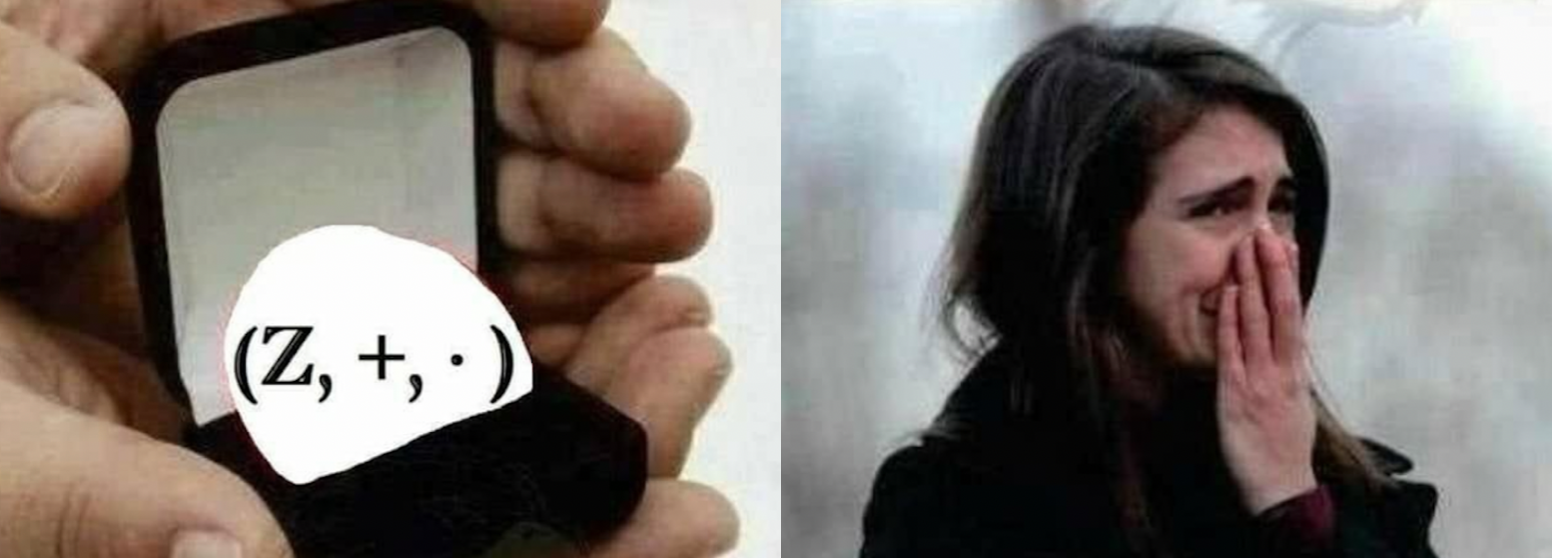
\includegraphics[width=1\textwidth]{imagenes/imagenes01/T01IM07.png}
	\end{figure}




	%\begin{figure}[H]
		%\centering
		%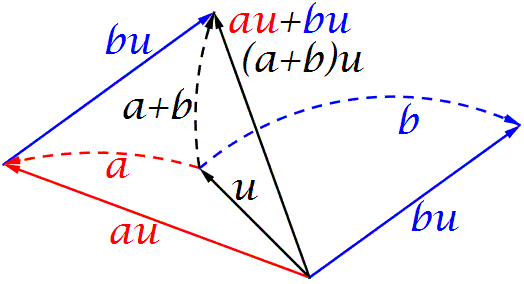
\includegraphics[width=0.5\textwidth]{imagenes/imagenes01/T01IM01.png}
		%\caption{Los dos problemas clásicos del cálculo: trazado de tangentes y áreas bajo curvas.}
	%\end{figure}
		
%varios párrafos encuadrados - explicaciones ad hoc
%\centering{
%\fbox{
%\parbox{0.95\textwidth}{
%varios
%
%$parrafos
%
%dentro
%}
%}
%}
% \justify


%\rotatebox{180}{\leftline{\textcolor{gris}{tararí}}}.